\documentclass{article}

\usepackage{graphicx}
\usepackage{tikz}
\usepackage{tikzsymbols}
\usetikzlibrary{calc,patterns,shapes.geometric}
\pagestyle{empty}
\usepackage[margin=0pt]{geometry}
\geometry{papersize={14in,12in}}

\def\centerarc[#1](#2)(#3:#4:#5){\draw[#1] ($(#2)+({#5*cos(#3)},{#5*sin(#3)})$) arc (#3:#4:#5);}

\begin{document}
	\begin{figure}
		\centering
		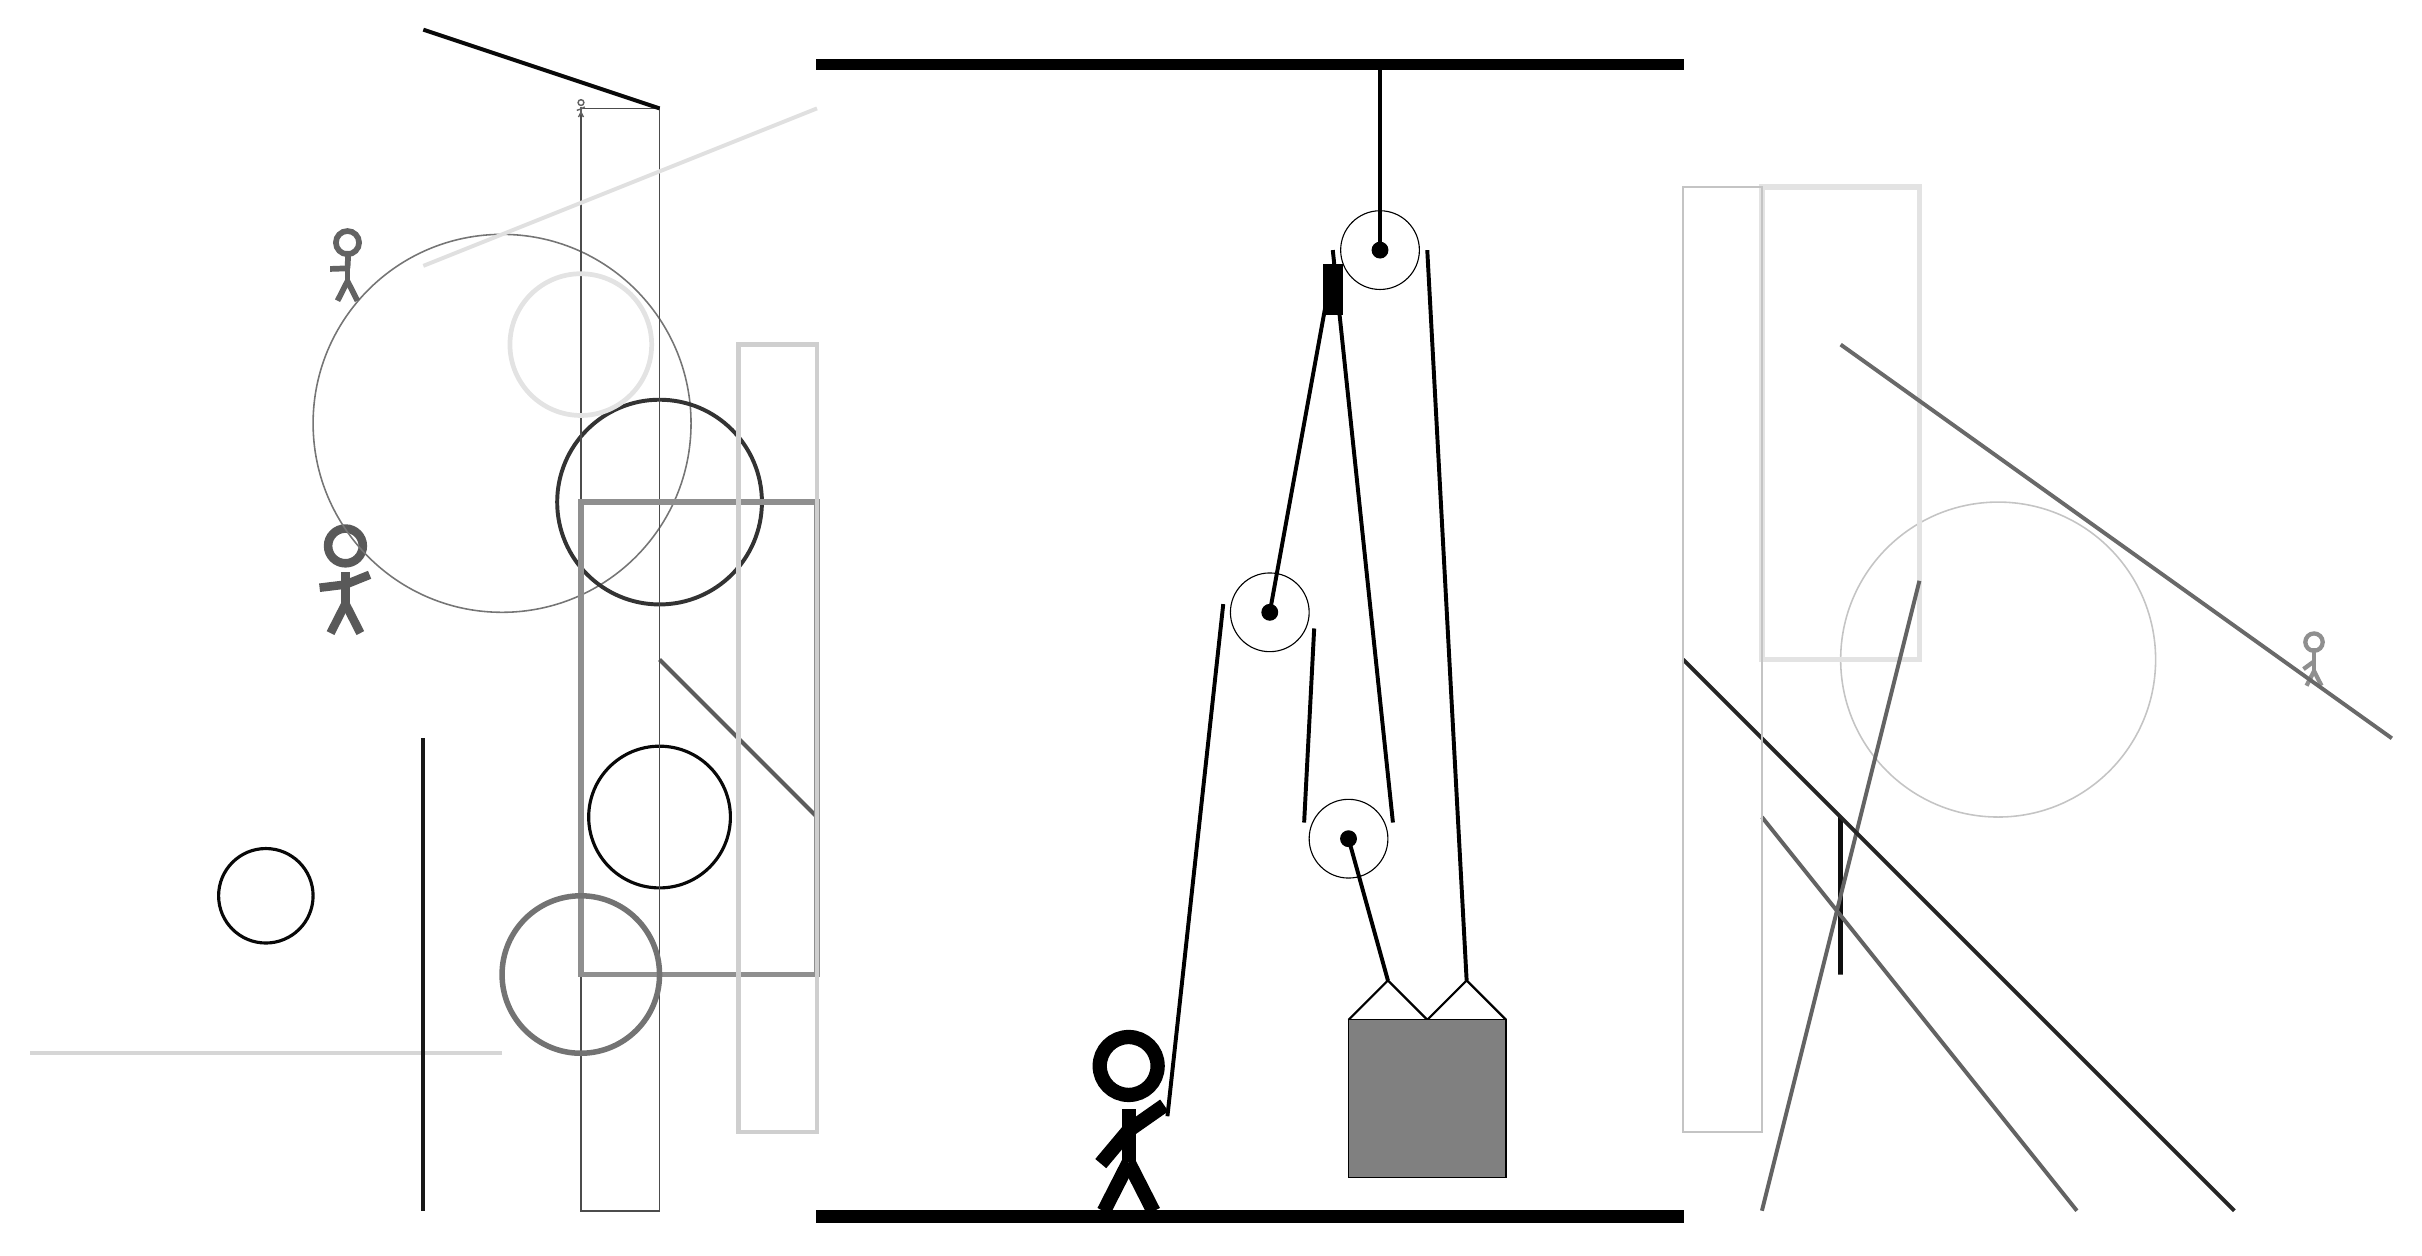
\begin{tikzpicture}
			%%%%% START %%%%%
			
			\draw[fill=black] (-6, 11.5) rectangle (5, 11.625);
			
			\node[line width=0.4mm, color=black!65] at (-12, 5) {\Strichmaxerl[6][7][22]};
			
			\node[line width=0.5mm, color=black!44] at (13, 4) {\Strichmaxerl[3][36][90]};
			\draw [line width=0.2mm, color=black!54](-10, 7) circle (2.4);
			\draw [line width=0.2mm, color=black!23](9, 4) circle (2.0);
			
			\draw[line width=0.5mm, color=black!16](-10, -1) -- (-16, -1);
			
			\draw[line width=0.7mm, color=black!94] (7, 0) rectangle (7, 2);
			\draw[line width=0.7mm, color=black!11] (6, 4) rectangle (8, 10);
			\draw[line width=0.5mm, color=black!61](8, 5) -- (6, -3);
			\draw [line width=0.5mm, color=black!80](-8, 6) circle (1.3);
			\draw[line width=0.5mm, color=black!64](-6, 2) -- (-8, 4);
			\draw [line width=0.4mm, color=black!97](-8, 2) circle (0.9);
			\draw[line width=0.5mm, color=black!61](10, -3) -- (6, 2);
			\draw[line width=0.2mm, color=black!70] (-8, 11) rectangle (-9, -3);
			
			\node[line width=0.5mm, color=black!62] at (-9, 11) {\Strichmaxerl[1][18][29]};
			\draw[line width=0.5mm, color=black!12](-11, 9) -- (-6, 11);
			\draw [line width=0.4mm, color=black!97](-13, 1) circle (0.6);
			
			\draw[line width=0.5mm, color=black!85](5, 4) -- (12, -3);
			
			\node[line width=0.3mm, color=black!61] at (-12, 9) {\Strichmaxerl[4][2][87]};
			\draw[line width=0.7mm, color=black!44] (-6, 6) rectangle (-9, 0);
			\draw[line width=0.2mm, color=black!23] (5, -2) rectangle (6, 10);
			\draw [line width=0.6mm, color=black!11](-9, 8) circle (0.9);
			
			\draw[line width=0.5mm, color=black!59](7, 8) -- (14, 3);
			
			\draw[line width=0.5mm, color=black!91](-11, 3) -- (-11, -3);
			\draw[line width=0.6mm, color=black!19] (-6, -2) rectangle (-7, 8);
			\draw[line width=0.5mm, color=black!97](-11, 12) -- (-8, 11);
			
			\draw [line width=0.7mm, color=black!55](-9, 0) circle (1.0);
			
			
			\draw (-0.25, 4.6) circle (0.5);
			\draw[fill=black] (-0.25, 4.6) circle (0.1);
			
			\draw (0.75, 1.725) circle (0.5);
			\draw[fill=black] (0.75, 1.725) circle (0.1);
			
			\draw (1.15, 9.2) circle (0.5);
			\draw[fill=black] (1.15, 9.2) circle (0.1);
			\draw[very thick] (1.15, 9.2) -- (1.15, 11.5);
			
			\draw[thick]  (0.75, -0.575) -- (1.25, -0.075) -- (1.75, -0.575) -- (2.25, -0.075) -- (2.75, -0.575);
			\draw[fill=black!50] (0.75, -0.575) rectangle (2.75, -2.575);
			
			\draw[line width=0.5mm] (-0.25, 4.6) -- (0.55, 9.0);
			\draw[line width=0.5mm, fill=black](0.45, 8.4) rectangle (0.65, 9.0);
			\draw[line width=0.5mm] (-1.55, -1.8) -- (-0.8409, 4.7042);
			\centerarc[line width=0.5mm](-0.25, 4.6)(-20:170:0.6);
			\draw[line width=0.5mm] (0.3138, 4.3948) -- (0.1862, 1.9302);
			\centerarc[line width=0.5mm](0.75, 1.725)(160:380:0.6);
			\draw[line width=0.5mm] (1.3138, 1.9302) -- (0.55, 9.2);
			\draw[line width=0.5mm](0.75, 1.725) -- (1.25, -0.075);
			\centerarc[line width=0.5mm](1.15, 9.2)(0:180:0.6);
			\draw[line width=0.5mm] (1.75, 9.2) -- (2.25, -0.075);
			
			\node at (-2, -1.9) {\Strichmaxerl[10][50][35]};
			
			\draw[fill=black] (-6, -3) rectangle (5, -3.15);
			
			%%%%% END %%%%%
		\end{tikzpicture}
	\end{figure}	
\end{document}